\documentclass{article}

% content/resources/templates/preamble.tex
\usepackage[margin=0.6in]{geometry}
\author{Milav Dabgar}
\usepackage{amsmath,amssymb,amsthm}
\usepackage{booktabs}
\usepackage{multirow}
\usepackage{xcolor}
\usepackage{tcolorbox}
\tcbuselibrary{breakable,skins}
\usepackage[colorlinks=true,linkcolor=blue]{hyperref}
\usepackage{titlesec}
\usepackage{enumitem}
\usepackage{tikz}
\usepackage{pgfplots}
\usepackage{circuitikz}
\usepackage[version=4]{mhchem}
\usepackage{longtable}
\usepackage{array}
\usepackage{float}
\usepackage{caption}
\usepackage{listings}

\lstset{
  basicstyle=\small\ttfamily,
  breaklines=true,
  breakatwhitespace=false,
  postbreak=\mbox{\textcolor{red}{$\hookrightarrow$}\space},
  float=false,
  numbers=left,
  numberstyle=\tiny\color{gray},
  numbersep=10pt,
  xleftmargin=2em,
  keywordstyle=\color{blue},
  commentstyle=\color{green!60!black},
  stringstyle=\color{purple},
  backgroundcolor=\color{gray!5},
  showstringspaces=false,
  tabsize=2,
  captionpos=b,
  keepspaces=true,
  columns=flexible
}

\pgfplotsset{compat=1.18}
\usetikzlibrary{shapes,arrows,positioning,calc,patterns,decorations.pathmorphing,decorations.markings,arrows.meta}

% Color scheme
\definecolor{headcolor}{RGB}{0,102,204}
\definecolor{keycolor}{RGB}{220,20,60}
\definecolor{solutioncolor}{RGB}{34,139,34}
\definecolor{mnemoniccolor}{RGB}{148,0,211}
\definecolor{codecolor}{RGB}{0,0,100}

% Spacing
\setlength{\parskip}{3pt}
\setlist[itemize]{nosep}
\setlist[enumerate]{nosep}

% Title formatting
\titleformat{\section}{\Large\bfseries\color{headcolor}}{\thesection}{1em}{}
\titleformat{\subsection}{\large\bfseries\color{headcolor}}{\thesubsection}{1em}{}

% Pandoc tightlist compatibility
\providecommand{\tightlist}{%
  \setlength{\itemsep}{0pt}\setlength{\parskip}{0pt}}

% Pandoc longtable compatibility
\newcounter{none}
\def\thenone{}


% content/resources/templates/english-boxes.tex

% Custom environments
\newtcolorbox{solutionbox}{
 breakable,
 enhanced,
 colback=solutioncolor!5!white,
 colframe=solutioncolor!75!black,
 fonttitle=\bfseries,
 title=Solution
}

\newtcolorbox{solutionboxnobreak}{
 colback=solutioncolor!5!white,
 colframe=solutioncolor!75!black,
 fonttitle=\bfseries,
 title=Solution
}

\newtcolorbox{keyformula}{
 breakable,
 enhanced,
 colback=keycolor!5!white,
 colframe=keycolor!75!black,
 fonttitle=\bfseries,
 title=Key Formula
}

\newtcolorbox{mnemonicboxenv}{
 breakable,
 enhanced,
 colback=mnemoniccolor!5!white,
 colframe=mnemoniccolor!75!black,
 fonttitle=\bfseries,
 title=Mnemonic
}

\newcommand{\mnemonicbox}[1]{%
  \begin{mnemonicboxenv}
    #1
  \end{mnemonicboxenv}
}


% Custom commands for GTU solutions
% This file defines semantic commands for consistent formatting

% Question command with automatic formatting
\newcommand{\question}[2]{%
  \section*{Question #1}%
  \textbf{#2}%
}

% OR question variant
\newcommand{\questionor}[2]{%
  \section*{Question #1 OR}%
  \textbf{#2}%
}

% Proper table environment with caption
\newenvironment{answertable}[1]{%
  \begin{table}[htbp]
  \centering
  \caption{#1}
}{%
  \end{table}
}

% Proper figure environment for diagrams
\newenvironment{answerdiagram}[1]{%
  \begin{figure}[htbp]
  \centering
  \caption{#1}
}{%
  \end{figure}
}

% Semantic markup for key terms
\newcommand{\keyword}[1]{\textbf{#1}}
\newcommand{\code}[1]{\texttt{#1}}
\newcommand{\classname}[1]{\texttt{#1}}
\newcommand{\methodname}[1]{\texttt{#1}}

% Proper quotation marks
\newcommand{\mnemonic}[1]{``#1''}


\title{Computer Networking (4343202) - Winter 2024 Solution}
\date{November 28, 2024}

\begin{document}
\maketitle

\questionmarks{1(a)}{3}{What is the Computer Network? Why it is important?}

\begin{solutionbox}
\textbf{Answer}:
A computer network is a collection of interconnected computing devices that can exchange data and share resources.

\textbf{Diagram:}

\begin{center}
\begin{tikzpicture}[node distance=2cm]
    \node [gtu block] (pc1) {Computer};
    \node [gtu block, right=of pc1] (pc2) {Computer};
    \node [gtu block, below=of pc1] (pc3) {Computer};
    \node [gtu block, right=of pc3] (pc4) {Computer};
    \draw [gtu arrow, <->] (pc1) -- (pc2);
    \draw [gtu arrow, <->] (pc1) -- (pc3);
    \draw [gtu arrow, <->] (pc3) -- (pc4);
    \draw [gtu arrow, <->] (pc2) -- (pc4);
\end{tikzpicture}
\captionof{figure}{Simple Computer Network}
\end{center}

\begin{itemize}
    \item \keyword{Resource sharing}: Enables sharing of printers, files, applications
    \item \keyword{Communication}: Facilitates information exchange between users
    \item \keyword{Scalability}: Allows networks to grow as needs increase
\end{itemize}
\end{solutionbox}

\begin{mnemonicbox}
\mnemonic{CSI - Connect, Share, Interact}
\end{mnemonicbox}

\questionmarks{1(b)}{4}{Define terms: 1) Web Server, 2)Encrypted data, 3)Hacking, 4)Client-server}

\begin{solutionbox}
\textbf{Definitions:}

\begin{center}
\captionof{table}{Network Terms}
\begin{tabulary}{\linewidth}{|L|L|}
\hline
\textbf{Term} & \textbf{Definition} \\ \hline
\textbf{Web Server} & Software/hardware that serves web content to clients using HTTP/HTTPS \\ \hline
\textbf{Encrypted Data} & Information converted to code to prevent unauthorized access \\ \hline
\textbf{Hacking} & Unauthorized access to computer systems through security vulnerabilities \\ \hline
\textbf{Client-Server} & Network model where centralized servers provide services to client computers \\ \hline
\end{tabulary}
\end{center}

\textbf{Client-Server Model:}

\begin{center}
\begin{tikzpicture}[node distance=2.5cm, auto]
    \node [gtu block] (client) {Client};
    \node [gtu block, right=of client] (server) {Server};
    
    \draw [gtu arrow, bend left] (client) to node {Request} (server);
    \draw [gtu arrow, bend left] (server) to node {Response} (client);
\end{tikzpicture}
\captionof{figure}{Client-Server Interaction}
\end{center}
\end{solutionbox}

\begin{mnemonicbox}
\mnemonic{WECHS - Web servers Encrypt data, Clients and Hackers use Servers}
\end{mnemonicbox}

\questionmarks{1(c)}{7}{Classify and explain the transmission media in detail.}

\begin{solutionbox}
\textbf{Transmission Media Types:}

\begin{center}
\captionof{table}{Transmission Media Classification}
\begin{tabulary}{\linewidth}{|L|L|L|L|}
\hline
\textbf{Category} & \textbf{Types} & \textbf{Characteristics} & \textbf{Applications} \\ \hline
\multicolumn{4}{|l|}{\textbf{Guided Media}} \\ \hline
Twisted Pair & UTP, STP & 100m range, 10Mbps-10Gbps & Office LANs \\ \hline
Coaxial Cable & Baseband, Broadband & 500m range, 10-100Mbps & Cable TV, Internet \\ \hline
Fiber Optic & Single/Multi-mode & Long distance, high speed & Backbone, WAN \\ \hline
\multicolumn{4}{|l|}{\textbf{Unguided Media}} \\ \hline
Radio Waves & WiFi, Cellular & Omnidirectional & Wireless networks \\ \hline
Microwaves & Terrestrial/Satellite & Line-of-sight & Point-to-point \\ \hline
Infrared & IrDA & Short-range & Remote controls \\ \hline
\end{tabulary}
\end{center}

\textbf{Diagram:}

\begin{center}
\begin{tikzpicture}[node distance=1.5cm]
    \node [gtu block, font=\bfseries] (media) {Transmission Media};
    \node [gtu block, below left=of media] (guided) {Guided (Wired)};
    \node [gtu block, below right=of media] (unguided) {Unguided (Wireless)};
    
    \node [below=0.2cm of guided, align=center, font=\footnotesize] {Twisted Pair\\Coaxial\\Fiber Optic};
    \node [below=0.2cm of unguided, align=center, font=\footnotesize] {Radio\\Microwave\\Infrared};
    
    \draw [gtu arrow] (media) -- (guided);
    \draw [gtu arrow] (media) -- (unguided);
\end{tikzpicture}
\captionof{figure}{Transmission Media Hierarchy}
\end{center}

\begin{itemize}
    \item \keyword{Guided media}: Physical paths for signal confinement
    \item \keyword{Unguided media}: Wireless transmission through air/space
    \item \keyword{Selection factors}: Cost, bandwidth, distance, environment
\end{itemize}
\end{solutionbox}

\begin{mnemonicbox}
\mnemonic{TCFRIM - Twisted pair, Coaxial, Fiber, Radio, Infrared, Microwave}
\end{mnemonicbox}

\questionmarks{1(c) OR}{7}{Explain WAN and MAN type of network.}

\begin{solutionbox}
\textbf{Comparison:}

\begin{center}
\captionof{table}{MAN vs WAN}
\begin{tabulary}{\linewidth}{|L|L|L|}
\hline
\textbf{Feature} & \textbf{MAN (Metropolitan)} & \textbf{WAN (Wide)} \\ \hline
\textbf{Coverage} & City-wide (5-50 km) & Country/Global (>50 km) \\ \hline
\textbf{Speed} & 10 Mbps - 10 Gbps & 1.5 Mbps - 1 Gbps \\ \hline
\textbf{Ownership} & Municipal/Telecom & Multiple organizations \\ \hline
\textbf{Examples} & City wifi, Campus Data & Internet, 4G/5G \\ \hline
\end{tabulary}
\end{center}

\textbf{Network Scope Diagram:}

\begin{center}
\begin{tikzpicture}[node distance=1cm]
    \node [gtu container, label=above:WAN (Global)] (wan) {
        \begin{tikzpicture}
             \node [gtu container, fill=white, label=center:MAN (City)] (man) {};
             \node [gtu container, fill=blue!10, minimum width=1.5cm, below=0.5cm of man, label=center:LAN] (lan) {};
        \end{tikzpicture}
    };
\end{tikzpicture}
\captionof{figure}{Network Scope Hierarchy}
\end{center}

\begin{itemize}
    \item \keyword{MAN}: Connects LANs within a city/metropolitan area
    \item \keyword{WAN}: Spans large geographical areas across cities/countries
    \item \keyword{Management}: WAN typically requires major service providers
\end{itemize}
\end{solutionbox}

\begin{mnemonicbox}
\mnemonic{SWIM - Size: WAN Is Massive compared to MAN}
\end{mnemonicbox}

\questionmarks{2(a)}{3}{Explain in detail: Transmission technology.}

\begin{solutionbox}
\textbf{Transmission Technologies:}

\begin{center}
\captionof{table}{Transmission Types}
\begin{tabulary}{\linewidth}{|L|L|L|}
\hline
\textbf{Technology} & \textbf{Description} & \textbf{Example} \\ \hline
\textbf{Point-to-Point} & Direct connection between two nodes & Leased line \\ \hline
\textbf{Broadcast} & Single channel shared by all nodes & Wireless LAN \\ \hline
\textbf{Multipoint} & Multiple devices share single link & Cable TV \\ \hline
\end{tabulary}
\end{center}

\begin{itemize}
    \item \keyword{Analog}: Continuous signal, susceptible to noise
    \item \keyword{Digital}: Discrete signal, more reliable
    \item \keyword{Baseband}: Single signal uses entire bandwidth (Ethernet)
    \item \keyword{Broadband}: Multiple signals share bandwidth (Cable TV)
\end{itemize}
\end{solutionbox}

\begin{mnemonicbox}
\mnemonic{ABP-DMB - Analog/Baseband Point-to-point; Digital/Multipoint Broadcast}
\end{mnemonicbox}

\questionmarks{2(b)}{4}{Draw and explain Star topology in detail.}

\begin{solutionbox}
\textbf{Star Topology Diagram:}

\begin{center}
\begin{tikzpicture}[node distance=2cm]
    \node [gtu block, fill=yellow!20] (hub) {Hub/Switch};
    \node [gtu state, above=of hub] (n1) {Node 1};
    \node [gtu state, below left=of hub] (n2) {Node 2};
    \node [gtu state, below right=of hub] (n3) {Node 3};
    
    \draw [gtu arrow, <->] (hub) -- (n1);
    \draw [gtu arrow, <->] (hub) -- (n2);
    \draw [gtu arrow, <->] (hub) -- (n3);
\end{tikzpicture}
\captionof{figure}{Star Topology}
\end{center}

\textbf{Analysis:}

\begin{center}
\captionof{table}{Star Topology Pros/Cons}
\begin{tabulary}{\linewidth}{|L|L|}
\hline
\textbf{Advantages} & \textbf{Disadvantages} \\ \hline
Easy installation & Single point of failure (Hub) \\ \hline
Simple troubleshooting & More cable required \\ \hline
Scalable & Higher cost due to central device \\ \hline
\end{tabulary}
\end{center}
\end{solutionbox}

\begin{mnemonicbox}
\mnemonic{CASE - Centralized, All connected, Simple expansion, Easy troubleshooting}
\end{mnemonicbox}

\questionmarks{2(c)}{7}{Draw and explain TCP/IP model.}

\begin{solutionbox}
\textbf{TCP/IP Model Layers:}

\begin{center}
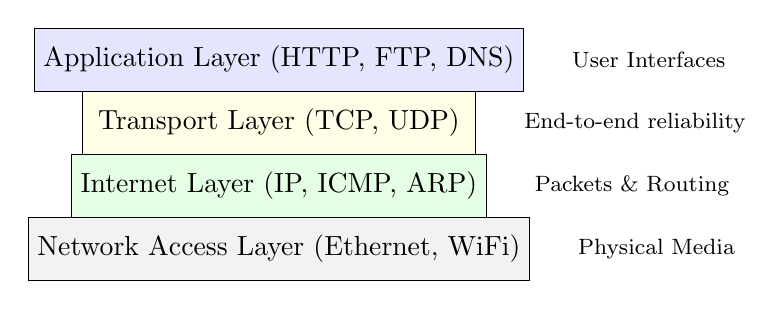
\begin{tikzpicture}[node distance=0cm, outer sep=0pt]
    \node [draw, rectangle, minimum width=5cm, minimum height=0.8cm, fill=blue!10] (app) {Application Layer (HTTP, FTP, DNS)};
    \node [draw, rectangle, minimum width=5cm, minimum height=0.8cm, below=of app, fill=yellow!10] (trans) {Transport Layer (TCP, UDP)};
    \node [draw, rectangle, minimum width=5cm, minimum height=0.8cm, below=of trans, fill=green!10] (inet) {Internet Layer (IP, ICMP, ARP)};
    \node [draw, rectangle, minimum width=5cm, minimum height=0.8cm, below=of inet, fill=gray!10] (net) {Network Access Layer (Ethernet, WiFi)};
    
    \node [right=0.5cm of app, align=left, font=\footnotesize] {User Interfaces};
    \node [right=0.5cm of trans, align=left, font=\footnotesize] {End-to-end reliability};
    \node [right=0.5cm of inet, align=left, font=\footnotesize] {Packets \& Routing};
    \node [right=0.5cm of net, align=left, font=\footnotesize] {Physical Media};
\end{tikzpicture}
\captionof{figure}{TCP/IP Stack}
\end{center}

\textbf{Layer Functions:}

\begin{itemize}
    \item \keyword{Application}: Interface between user applications and network
    \item \keyword{Transport}: Reliable data transfer between end systems
    \item \keyword{Internet}: Addressing and routing of packets
    \item \keyword{Network Access}: Physical hardware interface
\end{itemize}
\end{solutionbox}

\begin{mnemonicbox}
\mnemonic{ATNI - Application Talks, Network Internet Interfaces}
\end{mnemonicbox}

\questionmarks{2(a) OR}{3}{Draw and explain Bus topology in detail}

\begin{solutionbox}
\textbf{Bus Topology Diagram:}

\begin{center}
\begin{tikzpicture}[node distance=1.5cm]
    \draw [thick, double] (-3,0) -- (3,0) node[right] {Backbone Cable};
    \node [gtu state, below=0.5cm] (n1) at (-2,0) {Node1};
    \draw [thick] (-2,0) -- (n1);
    \node [gtu state, below=0.5cm] (n2) at (-0.5,0) {Node2};
    \draw [thick] (-0.5,0) -- (n2);
    \node [gtu state, below=0.5cm] (n3) at (1,0) {Node3};
    \draw [thick] (1,0) -- (n3);
    \node [gtu state, below=0.5cm] (n4) at (2.5,0) {Node4};
    \draw [thick] (2.5,0) -- (n4);
    \node [fill=black, minimum size=0.2cm] at (-3,0) {}; % Terminator
    \node [fill=black, minimum size=0.2cm] at (3,0) {}; % Terminator
\end{tikzpicture}
\captionof{figure}{Bus Topology}
\end{center}

\textbf{Analysis:}

\begin{itemize}
    \item \keyword{Advantages}: Simple layout, less cabling, low cost
    \item \keyword{Disadvantages}: Backbone failure stops all, difficult troubleshooting
    \item \keyword{Terminator}: Required at ends to prevent signal reflection
\end{itemize}
\end{solutionbox}

\begin{mnemonicbox}
\mnemonic{SLUE - Simple Layout, Uses less cable, Easy installation}
\end{mnemonicbox}

\questionmarks{2(b) OR}{4}{Explain Network Classification based on its architecture.}

\begin{solutionbox}
\textbf{Network Architectures:}

\begin{center}
\captionof{table}{Architecture Comparison}
\begin{tabulary}{\linewidth}{|L|L|L|}
\hline
\textbf{Architecture} & \textbf{Characteristics} & \textbf{Example} \\ \hline
\textbf{Peer-to-Peer} & Equal privileges, decentralized & torrents, home LAN \\ \hline
\textbf{Client-Server} & Centralized services & Enterprise networks \\ \hline
\textbf{Three-Tier} & Presentation, Logic, Data tiers & Web apps \\ \hline
\end{tabulary}
\end{center}

\textbf{Diagrams:}

\begin{center}
\begin{tikzpicture}[node distance=1.5cm]
    % P2P
    \node [gtu state, font=\tiny] (p1) {Peer};
    \node [gtu state, font=\tiny, right=of p1] (p2) {Peer};
    \draw [gtu arrow, <->] (p1) -- (p2);
    
    % Client-Server
    \node [gtu block, right=3cm of p2] (server) {Server};
    \node [gtu state, font=\tiny, below left=of server] (c1) {Client};
    \node [gtu state, font=\tiny, below right=of server] (c2) {Client};
    \draw [gtu arrow, <->] (c1) -- (server);
    \draw [gtu arrow, <->] (c2) -- (server);
    
    \node [below=0.2cm of p1] {P2P};
    \node [below=0.2cm of server] {Client-Server};
\end{tikzpicture}
\captionof{figure}{Architecture Models}
\end{center}
\end{solutionbox}

\begin{mnemonicbox}
\mnemonic{PCAN - Peer-to-peer, Client-server, Architecture Networks}
\end{mnemonicbox}

\questionmarks{2(c) OR}{7}{Explain classification of IP address.}

\begin{solutionbox}
\textbf{IP Classifications:}

\begin{center}
\captionof{table}{IP Addressing Classes}
\begin{tabulary}{\linewidth}{|L|L|L|L|}
\hline
\textbf{Class} & \textbf{Range (1st Octet)} & \textbf{Mask} & \textbf{Hosts} \\ \hline
\textbf{A} & 1 - 126 & 255.0.0.0 & 16M+ \\ \hline
\textbf{B} & 128 - 191 & 255.255.0.0 & 65,534 \\ \hline
\textbf{C} & 192 - 223 & 255.255.255.0 & 254 \\ \hline
\textbf{D} & 224 - 239 & N/A & Multicast \\ \hline
\textbf{E} & 240 - 255 & N/A & Reserved \\ \hline
\end{tabulary}
\end{center}

\textbf{Structure Diagram:}

\begin{center}
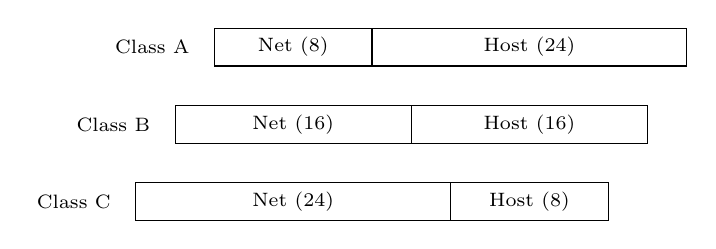
\begin{tikzpicture}[node distance=0cm, outer sep=0pt, font=\scriptsize]
    \node [draw, rectangle, minimum width=2cm] (a1) {Net (8)};
    \node [draw, rectangle, minimum width=4cm, right=of a1] (a2) {Host (24)};
    
    \node [draw, rectangle, minimum width=3cm, below=0.5cm of a1] (b1) {Net (16)};
    \node [draw, rectangle, minimum width=3cm, right=of b1] (b2) {Host (16)};
    
    \node [draw, rectangle, minimum width=4cm, below=0.5cm of b1] (c1) {Net (24)};
    \node [draw, rectangle, minimum width=2cm, right=of c1] (c2) {Host (8)};
    
    \node [left=0.2cm of a1] {Class A};
    \node [left=0.2cm of b1] {Class B};
    \node [left=0.2cm of c1] {Class C};
\end{tikzpicture}
\captionof{figure}{Classful Addressing Structure}
\end{center}

\begin{itemize}
    \item \keyword{Special Ranges}: Private IPs (10.x, 192.168.x), Loopback (127.0.0.1)
    \item \keyword{CIDR}: Newer classless routing replaces this legacy system
\end{itemize}
\end{solutionbox}

\begin{mnemonicbox}
\mnemonic{ABCDE - Address Blocks Categorized by Decreasing End-host counts}
\end{mnemonicbox}

\questionmarks{3(a)}{3}{What is full name of LAN? Explain it in detail.}

\begin{solutionbox}
\textbf{Definition:}
LAN stands for Local Area Network, a network confined to a limited geographic area.

\textbf{Diagram:}

\begin{center}
\begin{tikzpicture}[node distance=2cm]
    \node [gtu block] (switch) {Switch};
    \node [gtu block, left=of switch] (pc1) {Computer};
    \node [gtu block, right=of switch] (pc2) {Computer};
    \node [gtu block, above=of switch] (prn) {Printer};
    \node [gtu block, below=of switch] (pc3) {Computer};
    
    \draw [gtu arrow, <->] (switch) -- (pc1);
    \draw [gtu arrow, <->] (switch) -- (pc2);
    \draw [gtu arrow, <->] (switch) -- (prn);
    \draw [gtu arrow, <->] (switch) -- (pc3);
\end{tikzpicture}
\captionof{figure}{Local Area Network}
\end{center}

\textbf{Characteristics:}

\begin{center}
\captionof{table}{LAN Features}
\begin{tabulary}{\linewidth}{|L|L|}
\hline
\textbf{Characteristic} & \textbf{Description} \\ \hline
\textbf{Scope} & Building/Campus (1-2 km) \\ \hline
\textbf{Speed} & High (10 Mbps - 10 Gbps) \\ \hline
\textbf{Ownership} & Single organization/individual \\ \hline
\textbf{Media} & Twisted pair, Fiber, WiFi \\ \hline
\end{tabulary}
\end{center}
\end{solutionbox}

\begin{mnemonicbox}
\mnemonic{LOCAL - Limited in range, Owned by one entity, Connected devices, Access control, Low latency}
\end{mnemonicbox}

\questionmarks{3(b)}{4}{Write a short-note of Repeater.}

\begin{solutionbox}
\textbf{Repeater Function:}

\begin{center}
\begin{tikzpicture}[node distance=2cm]
    \node [gtu state, align=center] (weak) {Weak\\Signal};
    \node [gtu block, right=of weak] (repeater) {Repeater};
    \node [gtu state, right=of repeater, align=center] (strong) {Strong\\Signal};
    
    \draw [gtu arrow] (weak) -- (repeater);
    \draw [gtu arrow] (repeater) -- (strong);
    
    \node [below=0.5cm of repeater, font=\footnotesize] {Layer 1 Device};
\end{tikzpicture}
\captionof{figure}{Repeater Operation}
\end{center}

\begin{itemize}
    \item \keyword{Layer}: Physical Layer (OSI Layer 1)
    \item \keyword{Function}: Regenerates and amplifies signals
    \item \keyword{Purpose}: Extend network distance beyond cable limits
    \item \keyword{Limitation}: Cannot filter traffic or separate collision domains
\end{itemize}
\end{solutionbox}

\begin{mnemonicbox}
\mnemonic{RARE - Repeaters Amplify and Regenerate Electrical signals}
\end{mnemonicbox}

\questionmarks{3(c)}{7}{Write short note on FTP.}

\begin{solutionbox}
\textbf{File Transfer Protocol (FTP):}

\begin{center}
\begin{tikzpicture}[node distance=3cm]
    \node [gtu block] (client) {FTP Client};
    \node [gtu block, right=of client] (server) {FTP Server};
    
    \draw [gtu arrow, bend left] (client) to node[above] {Control (Port 21)} (server);
    \draw [gtu arrow, bend left] (server) to node[below] {Data (Port 20)} (client);
\end{tikzpicture}
\captionof{figure}{FTP Dual Connections}
\end{center}

\textbf{Key Features:}

\begin{center}
\captionof{table}{FTP Details}
\begin{tabulary}{\linewidth}{|L|L|}
\hline
\textbf{Feature} & \textbf{Description} \\ \hline
\textbf{Ports} & 21 (Control) and 20 (Data) \\ \hline
\textbf{Modes} & Active and Passive \\ \hline
\textbf{Auth} & Username/Password or Anonymous \\ \hline
\textbf{Data Types} & ASCII (text) and Binary \\ \hline
\end{tabulary}
\end{center}

\begin{itemize}
    \item \keyword{Dual Channel}: Separates commands from data transfer
    \item \keyword{Commands}: GET, PUT, LIST, DELETE, RENAME
    \item \keyword{Security}: Basic FTP is insecure; use FTPS/SFTP
\end{itemize}
\end{solutionbox}

\begin{mnemonicbox}
\mnemonic{CDATA - Control channel, Data channel, Active/passive modes, Transfer types, Authentication}
\end{mnemonicbox}

\questionmarks{3(a) OR}{3}{What is full name of PAN? Explain in detail.}

\begin{solutionbox}
\textbf{Personal Area Network (PAN):}

\begin{center}
\begin{tikzpicture}[node distance=1.5cm]
    \node [gtu state] (user) {User};
    \node [gtu block, above=of user] (phone) {Phone};
    \node [gtu block, right=of user] (laptop) {Laptop};
    \node [gtu block, left=of user] (watch) {Watch};
    \node [gtu block, below=of user] (buds) {Earbuds};
    
    \draw [dashed] (user) -- (phone);
    \draw [dashed] (user) -- (laptop);
    \draw [dashed] (user) -- (watch);
    \draw [dashed] (user) -- (buds);
\end{tikzpicture}
\captionof{figure}{PAN Ecosystem}
\end{center}

\begin{itemize}
    \item \keyword{Scope}: Very small (1-10 meters), centered on a person
    \item \keyword{Tech}: Bluetooth, Zigbee, NFC (Wireless); USB (Wired)
    \item \keyword{Use}: Data sync, audio streaming, wearables
\end{itemize}
\end{solutionbox}

\begin{mnemonicbox}
\mnemonic{PIPER - Personal, Individual, Proximity, Easy setup, Reduced range}
\end{mnemonicbox}

\questionmarks{3(b) OR}{4}{What is the importance of a Bridge? Write short-note on it.}

\begin{solutionbox}
\textbf{Bridge Operation:}

\begin{center}
\begin{tikzpicture}[node distance=2cm]
    \node [gtu block] (bridge) {Bridge};
    \node [gtu container, left=of bridge, label=below:Segment A] (segA) {Nodes};
    \node [gtu container, right=of bridge, label=below:Segment B] (segB) {Nodes};
    
    \draw [gtu arrow, <->] (bridge) -- (segA);
    \draw [gtu arrow, <->] (bridge) -- (segB);
    
    \node [below=0.5cm of bridge, font=\footnotesize] {Filters by MAC};
\end{tikzpicture}
\captionof{figure}{Network Bridge}
\end{center}

\begin{itemize}
    \item \keyword{Layer}: Data Link Layer (Layer 2)
    \item \keyword{Function}: Connects segments, filters traffic using MAC addresses
    \item \keyword{Benefit}: Reduces collision domains, reduces traffic
    \item \keyword{Types}: Transparent, Source-route
\end{itemize}
\end{solutionbox}

\begin{mnemonicbox}
\mnemonic{SELF - Segmentation, Extension, Learning addresses, Filtering traffic}
\end{mnemonicbox}

\questionmarks{3(c) OR}{7}{What is DSL? Explain its different types.}

\begin{solutionbox}
\textbf{Digital Subscriber Line (DSL):}

\begin{center}
\begin{tikzpicture}[node distance=2cm]
    \node [gtu block] (home) {Home Modem};
    \node [gtu block, right=3cm of home] (dslam) {ISP DSLAM};
    
    \draw [thick] (home) -- node[above] {Phone Line} (dslam);
    \node [below=0.5cm of home] {Data + Voice};
\end{tikzpicture}
\captionof{figure}{DSL Connection}
\end{center}

\textbf{DSL Types:}

\begin{center}
\captionof{table}{DSL Variants}
\begin{tabulary}{\linewidth}{|L|L|L|}
\hline
\textbf{Type} & \textbf{Name} & \textbf{Characteristics} \\ \hline
\textbf{ADSL} & Asymmetric & Faster download than upload (Home use) \\ \hline
\textbf{SDSL} & Symmetric & Equal speeds (Business use) \\ \hline
\textbf{VDSL} & Very High-bit-rate & Very fast, short distance \\ \hline
\textbf{HDSL} & High-bit-rate & T1/E1 replacement \\ \hline
\end{tabulary}
\end{center}

\begin{itemize}
    \item \keyword{Mechanism}: Uses higher frequencies on copper phone lines
    \item \keyword{Advantage}: Simultaneous voice and data, always-on
\end{itemize}
\end{solutionbox}

\begin{mnemonicbox}
\mnemonic{SAVHI - Symmetric, Asymmetric, Very high-bit-rate, High-bit-rate, ISDN DSL}
\end{mnemonicbox}

\questionmarks{4(a)}{3}{Explain an error control and flow control at data link layer.}

\begin{solutionbox}
\textbf{Data Link Controls:}

\begin{center}
\captionof{table}{Control Mechanisms}
\begin{tabulary}{\linewidth}{|L|L|L|}
\hline
\textbf{Mechanism} & \textbf{Purpose} & \textbf{Techniques} \\ \hline
\textbf{Error Control} & Detect/fix errors & CRC, Checksum, Retransmission (ARQ) \\ \hline
\textbf{Flow Control} & Prevent overflow & Stop-and-wait, Sliding Window \\ \hline
\end{tabulary}
\end{center}

\textbf{Flow Control Diagram:}

\begin{center}
\begin{tikzpicture}[node distance=2cm]
    \node [gtu state] (s) {Sender};
    \node [gtu state, right=of s] (r) {Receiver};
    
    \draw [gtu arrow, bend left] (s) to node[above] {Data} (r);
    \draw [gtu arrow, bend left, dashed] (r) to node[below] {Stop / ACK} (s);
\end{tikzpicture}
\captionof{figure}{Flow Control Concept}
\end{center}
\end{solutionbox}

\begin{mnemonicbox}
\mnemonic{SAFE - Stop-and-wait, Acknowledgment, Flow control, Error detection}
\end{mnemonicbox}

\questionmarks{4(b)}{4}{What is Firewall? Explain it in detail.}

\begin{solutionbox}
\textbf{Firewall Operation:}

\begin{center}
\begin{tikzpicture}[node distance=2cm]
    \node [gtu state] (inet) {Internet};
    \node [gtu block, fill=red!20, right=of inet] (fw) {Firewall};
    \node [gtu state, right=of fw] (lan) {Intranet};
    
    \draw [gtu arrow, <->] (inet) -- (fw);
    \draw [gtu arrow, <->] (fw) -- (lan);
    
    \node [below=0.5cm of fw, font=\footnotesize] {Allow/Block Rules};
\end{tikzpicture}
\captionof{figure}{Network Firewall}
\end{center}

\textbf{Types:}

\begin{itemize}
    \item \keyword{Packet Filtering}: Checks headers (IP/Port)
    \item \keyword{Stateful}: Tracks connection context
    \item \keyword{Application}: Inspects payload data
    \item \keyword{Next-Gen}: Integrated security features
\end{itemize}
\end{solutionbox}

\begin{mnemonicbox}
\mnemonic{PAPSI - Packet filtering, Application layer, Policies, Stateful inspection}
\end{mnemonicbox}

\questionmarks{4(c)}{7}{Compare IPV4 and IPV6.}

\begin{solutionbox}
\textbf{Comparison:}

\begin{center}
\captionof{table}{IPv4 vs IPv6}
\begin{tabulary}{\linewidth}{|L|L|L|}
\hline
\textbf{Feature} & \textbf{IPv4} & \textbf{IPv6} \\ \hline
\textbf{Size} & 32-bit (4.3B addresses) & 128-bit (Undecillion) \\ \hline
\textbf{Format} & Dotted Decimal & Hexadecimal with colons \\ \hline
\textbf{Header} & Variable (20-60B) & Fixed (40B) \\ \hline
\textbf{Security} & Optional (IPSec) & Built-in (IPSec) \\ \hline
\textbf{Checksum} & In header & Removed \\ \hline
\end{tabulary}
\end{center}

\textbf{Header Structures:}

\begin{center}
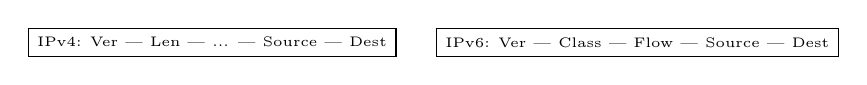
\begin{tikzpicture}[node distance=0.5cm, font=\tiny]
    \node [draw, rectangle, minimum width=3cm] (h4) {IPv4: Ver | Len | ... | Source | Dest};
    \node [draw, rectangle, minimum width=4cm, right=of h4] (h6) {IPv6: Ver | Class | Flow | Source | Dest};
\end{tikzpicture}
\captionof{figure}{Simplified Header Structure}
\end{center}

\begin{itemize}
    \item \keyword{Auto-config}: IPv6 supports stateless auto-configuration (SLAAC)
    \item \keyword{No NAT}: IPv6 restores end-to-end connectivity
\end{itemize}
\end{solutionbox}

\begin{mnemonicbox}
\mnemonic{SHAPE - Size, Header, Addressing, Performance, Extensibility}
\end{mnemonicbox}

\questionmarks{4(a) OR}{3}{What is an IP address? How it is used in network?}

\begin{solutionbox}
\textbf{IP Address Definition:}
A numerical identifier assigned to each device on a network for communication.

\textbf{Diagram:}

\begin{center}
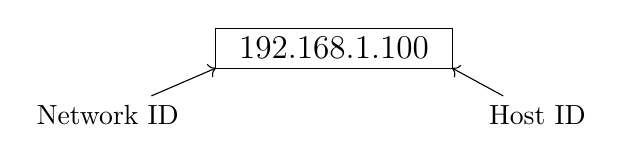
\begin{tikzpicture}[node distance=0cm, outer sep=0pt]
    \node [draw, rectangle, minimum width=3cm] (ip) {\large 192.168.1.100};
    \node [below left=0.5cm of ip] (net) {Network ID};
    \node [below right=0.5cm of ip] (host) {Host ID};
    
    \draw [->] (net) -- (ip.south west);
    \draw [->] (host) -- (ip.south east);
\end{tikzpicture}
\captionof{figure}{IPv4 Structure}
\end{center}

\begin{itemize}
    \item \keyword{Identification}: Uniquely names devices
    \item \keyword{Addressing}: Locates devices (like a postal address)
    \item \keyword{Routing}: Enables finding paths across networks
\end{itemize}
\end{solutionbox}

\begin{mnemonicbox}
\mnemonic{IRAN - Identification, Routing, Addressing, Network division}
\end{mnemonicbox}

\questionmarks{4(b) OR}{4}{Compare FDDI and CDDI.}

\begin{solutionbox}
\textbf{FDDI vs CDDI:}

\begin{center}
\captionof{table}{Technology Comparison}
\begin{tabulary}{\linewidth}{|L|L|L|}
\hline
\textbf{Feature} & \textbf{FDDI (Fiber)} & \textbf{CDDI (Copper)} \\ \hline
\textbf{Media} & Fiber Optic & Twisted Pair (Copper) \\ \hline
\textbf{Speed} & 100 Mbps & 100 Mbps \\ \hline
\textbf{Range} & Up to 200 km & ~100 meters \\ \hline
\textbf{Cost} & High & Low \\ \hline
\textbf{Topology} & Dual Ring & Dual Ring \\ \hline
\end{tabulary}
\end{center}

\textbf{Dual Ring Topology:}

\begin{center}
\begin{tikzpicture}[node distance=1.5cm]
    \node [gtu state] (n1) {1};
    \node [gtu state, right=of n1] (n2) {2};
    \node [gtu state, below=of n2] (n3) {3};
    \node [gtu state, left=of n3] (n4) {4};
    
    \draw [gtu arrow] (n1) -- (n2);
    \draw [gtu arrow] (n2) -- (n3);
    \draw [gtu arrow] (n3) -- (n4);
    \draw [gtu arrow] (n4) -- (n1);
    
    \draw [gtu arrow, dashed] (n1) -- (n4);
    \draw [gtu arrow, dashed] (n4) -- (n3);
    \draw [gtu arrow, dashed] (n3) -- (n2);
    \draw [gtu arrow, dashed] (n2) -- (n1);
\end{tikzpicture}
\captionof{figure}{Dual Counter-Rotating Rings}
\end{center}
\end{solutionbox}

\begin{mnemonicbox}
\mnemonic{FDDI Flies, CDDI Crawls (Distance wise)}
\end{mnemonicbox}

\questionmarks{4(c) OR}{7}{Draw and explain OSI reference model in detail.}

\begin{solutionbox}
\textbf{OSI Layered Model:}

\begin{center}
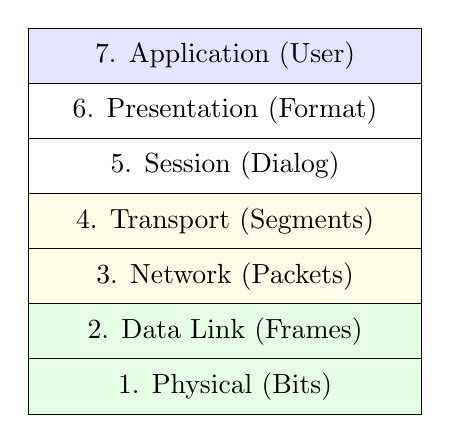
\begin{tikzpicture}[node distance=0cm, outer sep=0pt]
    \node [draw, rectangle, minimum width=5cm, minimum height=0.7cm, fill=blue!10] (l7) {7. Application (User)};
    \node [draw, rectangle, minimum width=5cm, minimum height=0.7cm, below=of l7] (l6) {6. Presentation (Format)};
    \node [draw, rectangle, minimum width=5cm, minimum height=0.7cm, below=of l6] (l5) {5. Session (Dialog)};
    \node [draw, rectangle, minimum width=5cm, minimum height=0.7cm, below=of l5, fill=yellow!10] (l4) {4. Transport (Segments)};
    \node [draw, rectangle, minimum width=5cm, minimum height=0.7cm, below=of l4, fill=yellow!10] (l3) {3. Network (Packets)};
    \node [draw, rectangle, minimum width=5cm, minimum height=0.7cm, below=of l3, fill=green!10] (l2) {2. Data Link (Frames)};
    \node [draw, rectangle, minimum width=5cm, minimum height=0.7cm, below=of l2, fill=green!10] (l1) {1. Physical (Bits)};
\end{tikzpicture}
\captionof{figure}{OSI 7-Layer Model}
\end{center}

\textbf{Analysis:}
\begin{itemize}
    \item \keyword{Encapsulation}: Data moves down layers, gaining headers.
    \item \keyword{Layers 1-3}: Media layers (Network specific).
    \item \keyword{Layers 4-7}: Host layers (Application specific).
\end{itemize}
\end{solutionbox}

\begin{mnemonicbox}
\mnemonic{All People Seem To Need Data Processing}
\end{mnemonicbox}

% Question 5
\questionmarks{5(a)}{3}{What is ISO? How it works in information security?}

\begin{solutionbox}
\textbf{Definition:}
ISO (International Organization for Standardization) creates global standards, including the ISO 27000 series for security.

\textbf{Functionality:}
\begin{itemize}
    \item \keyword{Standards}: ISO 27001 (ISMS), 27002 (Controls).
    \item \keyword{Framework}: Provides structured risk management (ISMS).
    \item \keyword{Compliance}: Organizations get certified for trust.
\end{itemize}
\end{solutionbox}

\begin{mnemonicbox}
\mnemonic{PRIMP - Policies, Risk assessment, Implementation, Monitoring, Process improvement}
\end{mnemonicbox}

\questionmarks{5(b)}{4}{Explain terms in detail for cryptography: 1) Encryption 2) Decryption}

\begin{solutionbox}
\textbf{Cryptography Concepts:}

\begin{center}
\begin{tikzpicture}[node distance=2.5cm]
    \node [gtu block] (plain) {Plaintext};
    \node [gtu block, right=of plain] (cipher) {Ciphertext};
    \node [gtu block, right=of cipher] (plain2) {Plaintext};
    
    \draw [gtu arrow] (plain) -- node[above] {Encrypt} node[below] {Key} (cipher);
    \draw [gtu arrow] (cipher) -- node[above] {Decrypt} node[below] {Key} (plain2);
\end{tikzpicture}
\captionof{figure}{Crypto Process}
\end{center}

\begin{itemize}
    \item \keyword{Encryption}: Converting plaintext to unreadable ciphertext to ensure confidentiality. Uses algorithms (AES, RSA).
    \item \keyword{Decryption}: Reverting ciphertext to plaintext using the correct key.
\end{itemize}
\end{solutionbox}

\begin{mnemonicbox}
\mnemonic{PACK-DUKE - Plaintext Algo Cipher Key - Decoding Using Key Extraction}
\end{mnemonicbox}

\questionmarks{5(c)}{7}{Write a short-note on 1) E-mail and 2) DNS}

\begin{solutionbox}
\textbf{1) E-mail System:}

\begin{center}
\begin{tikzpicture}[node distance=2cm]
    \node [gtu state] (sender) {Sender};
    \node [gtu block, right=of sender] (smtp) {SMTP Server};
    \node [gtu block, right=of smtp] (imap) {Mail Server};
    \node [gtu state, right=of imap] (rec) {Receiver};
    
    \draw [gtu arrow] (sender) -- (smtp);
    \draw [gtu arrow] (smtp) -- (imap);
    \draw [gtu arrow] (imap) -- (rec);
    
    \node [below=0.5cm of sender] {User Agent};
    \node [below=0.5cm of rec] {POP3/IMAP};
\end{tikzpicture}
\captionof{figure}{Email Flow}
\end{center}

\begin{itemize}
    \item \keyword{Protocols}: SMTP (Send), POP3/IMAP (Receive).
    \item \keyword{Components}: MUA (Client), MTA (Server).
\end{itemize}

\textbf{2) DNS (Domain Name System):}

\begin{center}
\begin{tikzpicture}[node distance=1.5cm]
    \node [gtu block] (root) {Root (.)};
    \node [gtu block, below left=of root] (com) {.com TLD};
    \node [gtu block, below right=of root] (org) {.org TLD};
    \node [gtu block, below=of com] (ex) {example.com};
    
    \draw [gtu arrow] (root) -- (com);
    \draw [gtu arrow] (root) -- (org);
    \draw [gtu arrow] (com) -- (ex);
\end{tikzpicture}
\captionof{figure}{DNS Hierarchy}
\end{center}

\begin{itemize}
    \item \keyword{Function}: Translates Domain Names -> IP Addresses.
    \item \keyword{Hierarchy}: Root -> TLD -> Authoritative.
    \item \keyword{Records}: A (IPv4), AAAA (IPv6), MX (Mail).
\end{itemize}
\end{solutionbox}

\begin{mnemonicbox}
\mnemonic{MAPS - Mail needs Addresses, Protocols, and Servers. HARD - Hierarchy, Addressing, Resolution, Distributed}
\end{mnemonicbox}

\questionmarks{5(a) OR}{3}{What do you mean by security topology and security zone?}

\begin{solutionbox}
\textbf{Concepts:}

\begin{center}
\begin{tikzpicture}[node distance=1.5cm]
    \node [gtu state] (net) {Internet};
    \node [gtu block, right=of net] (fw) {FW};
    \node [gtu class, right=of fw, fill=yellow!10] (dmz) {DMZ Zone};
    \node [gtu class, below=of fw, fill=green!10] (lan) {Private Zone};
    
    \draw [gtu arrow] (net) -- (fw);
    \draw [gtu arrow] (fw) -- (dmz);
    \draw [gtu arrow] (fw) -- (lan);
\end{tikzpicture}
\captionof{figure}{Security Zones}
\end{center}

\begin{itemize}
    \item \keyword{Security Topology}: The physical/logical layout of security controls (Firewalls, IDS).
    \item \keyword{Security Zone}: A network segment with a specific trust level (e.g., DMZ vs Internal).
\end{itemize}
\end{solutionbox}

\begin{mnemonicbox}
\mnemonic{TIPS - Topology Isolates and Protects Systems}
\end{mnemonicbox}

\questionmarks{5(b) OR}{4}{Write short-note on Voice and Video IP.}

\begin{solutionbox}
\textbf{VoIP / Video over IP:}

\begin{center}
\begin{tikzpicture}[node distance=2.5cm]
    \node [gtu state] (user1) {User};
    \node [gtu state, right=of user1] (user2) {User};
    
    \draw [gtu arrow, <->, dashed] (user1) -- node[above] {IP Network} node[below] {Data Packets} (user2);
    
    \node [below=0.5cm of user1, font=\tiny] {Digitize -> Packetize};
    \node [below=0.5cm of user2, font=\tiny] {Depacketize -> Analog};
\end{tikzpicture}
\captionof{figure}{Packet Voice/Video}
\end{center}

\begin{center}
\captionof{table}{Key Components}
\begin{tabulary}{\linewidth}{|L|L|}
\hline
\textbf{Component} & \textbf{Examples} \\ \hline
\textbf{Codecs} & G.711 (Voice), H.264 (Video) \\ \hline
\textbf{Protocols} & SIP (Setup), RTP (Transport) \\ \hline
\textbf{Requirements} & Low latency (QoS), High bandwidth \\ \hline
\end{tabulary}
\end{center}
\end{solutionbox}

\begin{mnemonicbox}
\mnemonic{CLEAR - Codecs compress, Latency matters, Encodes AV, Real-time transport}
\end{mnemonicbox}

\questionmarks{5(c) OR}{7}{What is IP security? Explain in detail.}

\begin{solutionbox}
\textbf{IPsec (Internet Protocol Security):}
A protocol suite for securing IP communications via authentication and encryption.

\begin{center}
\begin{tikzpicture}[node distance=2cm]
    \node [gtu block, fill=blue!10] (ipsec) {IPsec Suite};
    \node [gtu block, below left=of ipsec] (ah) {AH (Auth)};
    \node [gtu block, below=of ipsec] (esp) {ESP (Encrypt)};
    \node [gtu block, below right=of ipsec] (ike) {IKE (Keys)};
    
    \draw [gtu arrow] (ipsec) -- (ah);
    \draw [gtu arrow] (ipsec) -- (esp);
    \draw [gtu arrow] (ipsec) -- (ike);
\end{tikzpicture}
\captionof{figure}{IPsec Components}
\end{center}

\textbf{Components:}
\begin{itemize}
    \item \keyword{AH (Authentication Header)}: Integrity \& Auth. No encryption.
    \item \keyword{ESP (Encapsulating Security Payload)}: Encryption + Integrity + Auth.
    \item \keyword{IKE (Internet Key Exchange)}: Negotiates keys (SA).
\end{itemize}

\textbf{Modes:}
\begin{itemize}
    \item \keyword{Transport Mode}: Encrypts payload only (Host-to-host).
    \item \keyword{Tunnel Mode}: Encrypts entire packet (VPNs).
\end{itemize}
\end{solutionbox}

\begin{mnemonicbox}
\mnemonic{AVID TC - Auth, Verification, Integrity, Data protection, Transport/Tunnel modes, Confidentiality}
\end{mnemonicbox}

\end{document}
